\documentclass[12pt]{book} 

\usepackage{amsmath}
\usepackage{graphicx}
\usepackage{import}
\usepackage{amsfonts}
\usepackage{booktabs}

\setlength{\parindent}{0em}  % sets auto indent at new paragraph to none

\newcommand{\incfig}[1]{%
        \import{./figures/}{#1.pdf_tex}
}

\newcommand{\incimg}[2]{%
       \begin{figure}[h]
               \centering
               \includegraphics[scale = #2]{./figures/#1}
       \end{figure}
}

\title{\coursetitle\linebreak\lecturename}
\author{\\Cain Susko\\ 
           \\ \\ \\
      Queen's University 
    \\School of Computing\\} 

%=-=-=-=-=-title-=-=-=-=-=%
\newcommand{\lecturename}{Pipelines}
\newcommand{\coursetitle}{Computer Architecture}
%=-=-=-=-=-#####-=-=-=-=-=%

\begin{document}
\begin{titlepage}
        \maketitle
\end{titlepage}


\section*{Many Bits}
Last class, we went over how to implement sequential circuits with a single bit,
now we will be exploring how to implement circuits with many bits.

\subsection*{Memory Arrays}
Typically, memory is organized as a 2D array of memory cells. 
Consider the example of a 16x8 memory chip:
\incimg{memArr}{0.5}

when we read a row, we copy it to the buffer and we address the 8 bits, read them, and send them 
back to the CPU.

\subsection*{Register File}
Processors use many register to store temporary variables. Such a set of registers is calles a 
register file, and is built as a small, fast memory array. For example, a 32-register, 32-bit, 
register file with:
\begin{itemize}
        \item 2 read ports
        \item 1 write port
        \item a write-enable control
\end{itemize}
\incimg{regFile}{0.5}

\section*{Pipelining}
The idea of pipelines is that we will organize our instructions and their execution and instead 
of having a single instuction being executed we can have many executed at the same time. this is
how modern processors work.

\paragraph{Processing an Instruction}
Processing an instruction requires numerous operations. These operations can be organized in 
\textit{phases}:
\begin{enumerate}
        \item fetch
        \item decode
        \item execute
        \item memory
        \item write back
        \item PC update
\end{enumerate}
 This can be represented visually as:
 \incimg{process}{0.7}

 \subsection*{Fetch}
goes to memory, gets data, prepares components, and sends it on to be decoded.
 The fetch operation uses the $PC$ as the address. It then reads bytes of instruction
 from memory and prepares a new $PC$, $valP$
 \incimg{fetch}{0.5}

 \subsection*{Decode}
 The decode then uses instructions and function codes to control downstream harware. It Addresses
 into the register file to read or write values.
 \incimg{decode}{0.5}

 \subsection*{Execute}
 This part does the arithmatic logic or computation from the decode step. it also sets the 
 codes $Cnd$ which contains the effective address, the stack pointer, and the conditional moves
 and jumps.
\incimg{execute}{0.5}

\subsection*{Memory}
the memory is contained at $Addr$. It reads from memory, returning $ValM$ and writes $Data$
to memory.
\incimg{memory}{0.5}

\subsection*{Write Back}
 Take the computed value $valE$ and / or value loaded from memeory $ValM$ and write into the 
 register file. This operation is addressed by $dstE$ and $dstM$
 \incimg{writeback}{0.5}

 this is to take a computed value and save it back to the register.
 \pagebreak

 \subsection*{PC Update}
 This is to handle the different branches (if there are any) within the program.
 \incimg{PCupdate}{0.5}

 where PC update takes the input:
 \begin{itemize}
         \item the sequential $valP$
         \item the absolute adress read from memory
         \item the relative or effective address
         \item branching condition
 \end{itemize}

 \section*{Computation Pipelines}
 The whole process described above is what is known as Computation\\Pipeline. 
 An example of a pipeline in the physical world is a car production line.
 \pagebreak

 A 3-stage pipeline can be visually represented as:
 \incimg{3pipe}{0.5}

 Note: the data is stored between stages in registers, which are all controlled by the same clock. 
 so Pipelining is more accurate but uses more memory.

 A closer look at this pipelined circuit we can Observe:
 \begin{figure}[h]
         \centering
         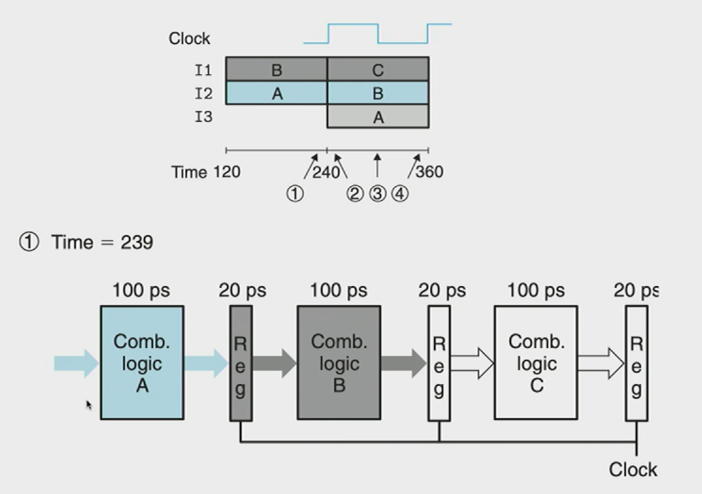
\includegraphics[scale=0.5]{./figures/close1.png}
         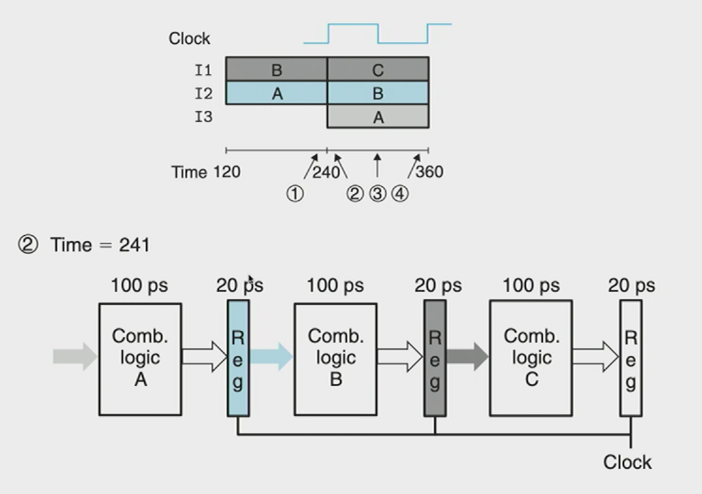
\includegraphics[scale=0.5]{./figures/close2.png}
 \end{figure}
 \begin{figure}[h]
         \centering
         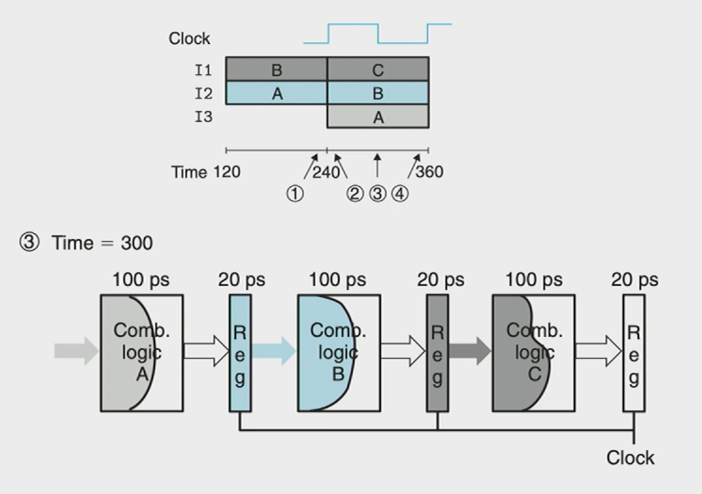
\includegraphics[scale=0.5]{./figures/close3.png}
         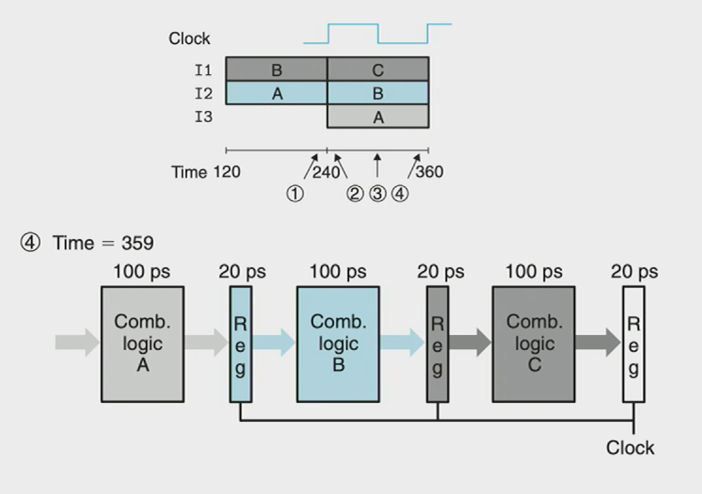
\includegraphics[scale=0.5]{./figures/close4.png}
 \end{figure}
 %\incimg{close1}{0.3}
 %\incimg{close2}{0.3}
 %\incimg{close3}{0.3}
 %\incimg{close4}{0.3}

\pagebreak
 \section*{Un-Pipelined Architecture}
 An example of a architecture that does not use pipelining is the following:
 \incimg{nopipe}{0.5}

 \section*{Limitations of Pipelining}
 There are many structural hazards that that one can encounter when implementing pipelined
 computing: like when 2 instructions need the same harware resources.

 Data hazards arise when one instruction depends on a value produced by a preceding instructions
 still in the pipeline.

 Control hazards include if an instruction should be executed needs a control decision by
 a preceeding instruction.

 Some solutions include:
 \begin{itemize}
         \item sheduling: programmer explicilty avoids 
         \item stall: suspending subsequent instruction
         \item duplicate: more hardware
         \item forward: allow data to bypass certain hardware units for early availablity
         \item speculate: guess the problem and kill speculative results if incorrect
 \end{itemize}
 \pagebreak

 \paragraph{Uninform Partitioning}
if the logic circuits are not evenly distrubuted over time (non-uniform partitioning)
, then the time of setion within the circuit must be allocated as the largest 
time within the for a section within the circuit. This can be seen
more clearly in the following diagram:
\incimg{limits}{0.5}
 
Note: we calculate the throughput by the equation:
\[TP = \frac{S}{d}\]
where $S$ is the number of steps or circuits and $d$ is the delay (ammount of time to execute)
 for the circuit.

 \paragraph{Deep Pipelining}
 When one implements a deep (more than 10 sections)
 pipelining structure. Because pipelining requires a register between each section, the returns
 from pipelining is diminished.

\end{document}

